\documentclass[a4paper,titlepage,12pt]{article}
\usepackage{parskip}
\usepackage{graphicx}
\usepackage{hyperref}
\hypersetup{
	hidelinks,
	pdfauthor=Delan Azabani; Callum Boyd; Jason Giancono; Robert Lai;
	          Luke Mercuri; Jasmine Quek; Kye Russell,
	pdftitle=Project Design and Management 300: FreedomSpace
}
\let\stdsection\section
\renewcommand\section{\newpage\stdsection}

\title{Project Design and Management 300\\FreedomSpace}
\date{June 1, 2014}
\author{
	To the Moon \\
	\hspace{10 mm} \\
	Delan Azabani \\
	Callum Boyd \\
	Jason Giancono \\
	Robert Lai \\
	Luke Mercuri \\
	Jasmine Quek \\
	Kye Russell \\
}

\pagenumbering{gobble}

\begin{document}

\maketitle
\pagenumbering{roman}
\tableofcontents
\newpage
\pagenumbering{arabic}

\section{(TODO: Jason) Abstract}

\section{Introduction and objectives}

The use of computers and information technology has increasingly become an
integral factor in research at universities. While the technology and its role
has increased, Curtin University still uses traditional methods such as paper
forms for allocating storage for research projects. In order for us to keep up
with the increasing demand of information technology services, many of these
traditional methods should be digitised and automated.

In order to eliminate this needless paperwork and bureaucracy, Curtin
University could implement a web-based portal for staff members to request and
allocate storage space for each project. This would reduce time loss in the
turnaround caused by waiting for requests, improve the efficacy of record
maintenance and offer extra opportunities for Curtin University to analyse and
optimise its data storage infrastructure.

\subsection{Objectives}

The objective of this project is to create a prototype of a web-based portal
for managing storage space requests at Curtin University. This will allow us to
demonstrate the concept to the stakeholders and refine it as needed. The
prototype isn't required to have the complete functionality, however the user
experience should be complete. The prototype should focus on user experience,
with usability being the main measure of success, as many staff members may not
be proficient with the use of technology.

\subsection{Scope}

The scope of the project will include gathering the user requirements of the
system, designing the user experience of the system and implementing a
prototype of this user experience. Actual functionality and requirements
regarding integration with Curtin University's information systems is outside
the scope of this project, and will depend on the reception of the prototype by
Curtin University's information technology department.

\subsection{Limitations}

The project has not been provided with a budget; all software dependencies must
be freely available, and all hardware must be sourced from group members and/or
computing resources provided by Curtin University.

The prototype will be developed on academic versions of the Visual Studio 2013
Professional integrated development environment, which means that no part of
this prototype may be deployed commercially.

The developers will not have access to Curtin University's LDAP directory
service and other information systems. This means that the prototype's main
focus will be on the user experience and the backend which facilitates that.
Enhancements such as integration with learning management systems and directory
services will be features likely available in a final product but will not be
represented in the prototype.

There are only twelve weeks to complete the entire project, including the
solicitation of requirements and user testing. Developers will also provide
different sets of skills, while being restricted by different unit timetables.

\subsection{Approach}

Our team is developing the prototype using the Scrum methodology. First the
Product Backlog is decided upon --- each item is allocated a priority, then
a subset of the user stories are chosen to be completely designed, implemented
and tested for each sprint. The team meets before and after each sprint to
discuss how the sprint went, as well as what needs to be completed in the next
sprint. This allows us to efficiently adapt to any issues with our
requirements.

\subsection{Structure}

This report will guide us through the background which has led to this project,
the requirements which have been decided upon for the prototype, the design of
the web-based portal and the process used during development of this project.

\section{Background}

\subsection{Initial project management approach}

(TODO: Gantt chart)

Our solution approach was to first prioritise the user stories given, so that
vital functionality would be implemented in early sprints. Shortly afterwards,
the team had a meeting to discuss the various permissions of the different user
account roles. In this meeting we made a permissions table so as to clear up
any confusion of the various user privileges.

The overarching approach was to figure out the solutions for the larger
problems as a group, and then to allocate tasks to be solved by assorted group
members by the end of the next sprint.

\subsection{(TODO: Jasmine) Tools considered for development}

\subsection{(TODO: Jasmine) User interface mockups}

\section{Product backlog}

Our first goal with user stories was to divide them into three groups
representing their priority for completion, with `1' being the highest and `3'
being the lowest. In the highest priority group we placed stories that we
believed to be related to core parts of the system. The second group were
stories that enhanced the core functionality of the system and added features
and other useful tools for the users. The lowest priority group were stories
that enhanced ease of access and usability as well as features that were not
core functionality.

In the first priority tier of user stories, we placed any stories relating to
authentication and user access levels. We felt that this was core to the system
because the users would have different permissions and access. There were quite
a few stories relating to logging in and being able to perform their functions
from that. Out of the seven user stories that were decided to be `priority
one', three were relating to login functions.

\begin{itemize}
	\item As an administrator, I want to login so that I can review and
	      approve requests;
	\item As a user, I want to login so that I can perform appropriate
	      functions applicable to my role; and
	\item As an approver, I want to login so that I can approve storage
	      requests.
\end{itemize}

In the first story we understand that the administrators of the system want to
be able to log in and approve requests. From this we can assume that they want
to be able to log in so that they will be able to have access to this feature,
not just anyone.

(TODO: insert login screen here)

We can further assume that this is also related to wanting some level of system
and user security so that only authorised personnel have access to requests.
This is also seen in the third story where the approver wants to be able to log
in to approve requests. From this we can see that approving requests is a
privileged feature and only these two types of users are able to do this.

The second user story shows that all users do want to be able to log in and
perform functions applicable to their role. This can be expanded to users want
to be able to log in and only see functions related to their own role,
therefore only displaying functions that they can use. From this assumption we
can work out that users only want to see what they can do and they don't want
to see everything else.

(TODO: insert screenshots of different user roles)

While this may seem like an ease of use story it is important to make sure that
all users can log in as soon as the first part of the working system is
complete; therefore this was classified as a first priority story.

\begin{itemize}
	\item As a principal investigator, I want to submit a storage request
	      so that I can have access to storage space for a research
	      project;
	\item As a user, I want to view a list of my storage spaces so that I
	      know my access level for my research projects;
	\item As an administrator, I want to approve a request so that storage
	      can be provisioned, expanded or access permissions changed; and
	\item As an approver, I want to review and approve a storage request so
	      that storage can be provisioned.
\end{itemize}

These four stories are the remainder of the tier one user stories. All four of
them relate to storage access; as this system is about managing access to
storage for researchers, it is very important that they are completed first.

The first story is about the principal investigator, which is the role of the
person who wants to have the storage set for their project. From this first
story we can gather that principal investigators want to be able to easily
request storage spaces as this is a key part of their role.

The second story can be split into two parts, the first part being that users
want to be able to see their storage spaces. This is a critical function of the
system because there is no point to having storage spaces if no one can see
them. The second part could very easily be forgotten due to the significance of
the first part and that is that the users also want to know their access levels
for these projects that have space allocated.

(TODO: picture of storage spaces)

The third story gives insight on what is wanted from the system in terms of
changing the storage of users. From this we can understand that administrators
want to be able to change the permissions, expand and approve storage. This
means the system needs to be able to dynamically set storage and user
permissions to add in or remove users' access to storage spaces. This was
classified as a high priority because it is a core part of the system that
access is granted and only to those who are approved.

The fourth story is quite similar to the third in that it is about approving
storage requests, which is why it is grouped with it. However it also helps
define the roles of administrator and approver, because from this story we can
see that only administrators want to be able to change permissions and expand
storage, where approvers only want to be able to approve as their name would
suggest.

What we learned from this first set stories is that we need to have a
well-defined set of rules of user permissions. From the user stories we know
that each user has a role within a project and that while some of their roles
do overlap or some functions they are all different. These user levels and
roles help define what users are allowed to do and access within the system.
Due to the key nature of system integrity we decided to come up with a diagram
of user permission levels for all the user types. This was used throughout the
design phase to create the different user logins in the system.

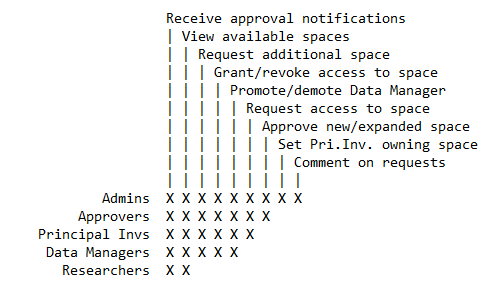
\includegraphics{../permissions.png}

For the second level of user stories we see a lot more stories about
collaboration and changing user access levels for the existing storage spaces.

\begin{itemize}
	\item As a data manager, I want to grant other researchers access to my
	      storage space so that I can collaborate with others;
	\item As a data manager, I want to submit additional storage requests
	      so that I can store more research data in my storage space;
	\item As a principal investigator, I want to grant other researchers
	      access to my storage space so that I can collaborate with others;
	\item As a principal investigator, I want to grant other researchers
	      data manager level access for my storage space so that they can
	      submit administrative requests; and
	\item As a principal investigator, I want to submit additional storage
	      requests so that I can store more research data in my storage
	      space.
\end{itemize}

From the first two stories we see a new user role, the data manager, which is a
user who controls the data and access of the projects. From the first of these
stories we can see that the data managers need to be able to control who has
access to their storage spaces which they want to use for collaboration. We
also see that in the third story the principal investigators want to be able to
grant other researches access to their storage spaces as well.

This pattern of data manager and principal investigator having very similar
stories continues again when we see that they both want to be able to request
more storage space for their projects. While most storage requests were in the
first priority group of user stories these ones are in the second priority
group because they are requesting additional storage which isn't a critical
feature.

The fourth story provides a good insight into the power of the principal
investigator as he wants to be able to create data managers from researchers.
This functionality is important because it allows the system to be mostly run
by users in their own project rather than having the global administrators set
roles for each project which could become a large amount of work if the system
is used across a large user base.

There were two more user stories that were set as priority two.

\begin{itemize}
	\item As an administrator, I want to change the principal investigator
	      for a storage space to replace the existing principal
	      investigator; and
	\item As an approver, I want to view a list of all storage requests so
	      that I am aware of all requests by principal investigators in my
	      faculty.
\end{itemize}

From this first story we see that administrators need to have the power to
change principal investigators of storage spaces. This is important because if
a principal investigator doesn't do their job properly it could be damaging to
the project. This also helps us better define the role of the administrators by
giving more insight into their needs.

The second story helps us understand the position of approvers within the
company because of they want to be able to see faculty based requests we can
understand that approvers would be a high position within the faculty and need
to see what researchers within the faculty need. This also helps show us that
the user classes we create must have a faculty identifier somewhere so that
this story can be met.

The third and final group of user stories were the stories we decided were the
lowest priority to complete in the system. These were features and functions
that did not have much of an impact on the functionality but were more for ease
of use.

\begin{itemize}
	\item As a data manager, I want to revoke an existing researcher's
	      access to my storage space so that they can't access my data;
	\item As a principal investigator, I want to revoke an existing
	      researcher's manager level access for my storage space so that
	      they cannot submit administrative requests;
	\item As a principal investigator, I want to revoke existing
	      researchers' access to my storage space so that they can't access
	      my data; and
	\item As a researcher, I want to receive email notification when my
	      access to a storage space is revoked so that I am aware that I
	      can no longer access it.
\end{itemize}

There were quite a few user stories relating to revoking access of a researcher
either to a space or of their administrative powers of that space. We felt that
these would definitely not be needed to demonstrate the product in the few
sprints and that there would be no point doing before researchers could be
added.

These user stories are much straighter forward than the earlier stories because
they are relating to simple functions that help with the maintainability of the
software. There is not more to be read out of the first three stories other
than the different high level role users want to be able to remove researchers
from their projects. It is a simple request and not a hard feature to implement
which is why it was pushed back to the lowest priority.

The fourth user story in this set is a bit different though because it is from
the researcher who wants to be notified about being removed from the storage
space. Email notifications were something that we decided did not need to be
down until all of the core functionality is in and working properly. So all
email and notification stories were placed in to the lowest priority group.

\begin{itemize}
	\item As a data manager, I want to receive email notifications so that
	      I am aware that requests have been completed;
	\item As a principal investigator, I want to receive email
	      notifications so that I am aware that requests have been
	      completed; and
	\item As a researcher, I want to receive email notifications when I am
	      granted access to a storage spaces so that I can access the data.
\end{itemize}

All of these stories are about email notifications for features that were
requested in higher priority stories. From these though we see that the system
does need to be able to sync to a mail server to deliver the email and that all
users need to register an email with their account.

One of the notification requests however was different, `As an administrator, I
want to send appropriate notifications so that users can start using their
storage spaces.' From this story we need to create a way for administrators to
be able to send notifications to users. This story in particular did not
however mention what kind of notification should be sent so it was up to us to
decide how best to send a notification.

\begin{itemize}
	\item As an administrator, I want to view a list of requests by
	      submission date so that I can review them chronologically; and
	\item As an approver, I want to view a list of all storage spaces for
	      my faculty so that I can determine storage space allocated for my
	      faculty.
\end{itemize}

These two stories show that the high level users want to be able to list
submission requests and have the sorted in a particular way. This meant that
some sort of algorithm would need to be implemented to sort them, we the first
story also refers to submission date which none of the others do which may have
not been stored otherwise. Although similar there are other stories that make a
note of faculty so it would be a bit more obvious to store which faculty a
project is part of.

The final user stories are about requests for storage. 

\begin{itemize}
	\item As a data manager, I want to view the status of my request so
	      that I know its progress;
	\item As a principal investigator, I want to view the status of my
	      request so that I know its progress; and
	\item As an administrator I want to add a comment to a request so that
	      I can highlight any special requirements or additional
	      information related to the request.
\end{itemize}

These stories show that users want to be able to see the status of their
requests so they can then follow up with administrators personally if need be.
The third story here does ask for something a bit different though and that is
the ability to add comments to requests. This does require adding on some extra
functionality, however as a group we decided that it was not core functionality
and did not need to be put in until all of the core features and functions were
added.

For the product backlog we ended up with seven user stories being classified as
highest priority, these were the core functions and features of the system.
There were six user stories as medium priority which was mostly usability
features such as increased user control. The lowest priority group had thirteen
user stories although as explained above many of these were the same story from
different users and most of them were increased user control or notification
requests.

\section{Sprint documentation}

\subsection{Sprint 1 planning}

The user stories that were chosen for the first sprint were the user stories
with the greatest importance, serving as the metaphorical foundations of the
project. To do this we rearranged and categorised the user stories by their
importance, access level requirements, and dependencies to yield the tasks
which required the lowest level of requirements to complete first. The first
sprint should contain everything that would be mandatory in the second and
third sprints, namely:

\begin{itemize}
	\item As an administrator, I want to log in so that I can review and
	      approve requests;
	\item As a principal investigator, I want to submit storage requests so
	      that I can have access to a storage space for a research project;
	\item As a user, I want to log in so that I can perform appropriate
	      functions applicable to my role;
	\item As a user, I want to view a list of my storage spaces so that I
	      know my access level for my research projects;
	\item As an administrator, I want to approve a request so that storage
	      can be provisioned, expanded or access permissions changed;
	\item As an approver, I want to log in so that I can approve storage
	      requests; and
	\item As an approver, I want to review and approve a storage request so
	      that storage can be provisioned.
\end{itemize}

These user stories are what we collectively prioritised as the most important
tasks to complete before any other parts of the project can be undertaken.

The breakdown that we had planned for the project as a whole was to correlate
all user stories to a number depending on what required the least functionality
as well as which user stories required others to be completed before they could
be implemented. By doing this, we managed to organise all of the user stories
into three groups, which ideally would be allocated to each sprint. The first
sprint would involve everything on the lowest level, which includes logging
into the website, viewing spaces and reviewing requests as the users with the
highest levels of access permissions.

With this we estimated that it would take approximately two weeks. This would
give us enough time for the group to orientate and establish suitable
communications between all members. After that, we would be able to work
smoothly throughout the project. Within this fortnight, one week will be set
aside to create the user login system and have it operational, then three days
will be allocated to implement the viewing of lists and reviewing of storage
requests. The remaining four days would go towards fixing defects and polishing
what has been done thus far, in addition to working on other projects.

\subsection{Sprint 1 review}

In the first sprint, the user stories decided upon were fairly ambitious. As a
group we completed a number of allocated user stories including:

\begin{itemize}
	\item As an administrator, I want to log in so that I can review and
	      approve requests;
	\item As a user, I want to log in so that I can perform appropriate
	      functions applicable to my role; and
	\item As an approver, I want to log in so that I can approve storage
	      requests.
\end{itemize}

These user stories overlapped in functionality and so were considered as one
single task, which was completed by Delan.

\begin{itemize}
	\item As a principal investigator, I want to submit storage requests so
	      that I can have access to storage space for research projects;
	\item As a data manager, I want to submit additional storage requests
	      so that I can store more research data in my storage space; and
	\item As a principal investigator, I want to submit additional storage
	      requests so that I can store more research data in my storage
	      space.
\end{itemize}

As with the login user stories, the above stories were considered to be one
single task due to the similarity in their functionality, and they were
completed by Kye.

\begin{itemize}
	\item As a user, I want to view a list of my storage spaces so that I
	      know my access level for my research projects; and
	\item As an approver, I want to view a list of all storage spaces for
	      my faculty so that I can determine storage space allocated to my
	      faculty.
\end{itemize}

This task was not completed in its entirety at this stage but the majority of
it had been completed and was ready for presentation. Completion of this task
was a joint effort between Jason and Kye.

There were also planned user stories that at this point were not yet complete,
such as:

\begin{itemize}
	\item As an administrator, I want to approve a request so that storage
	      can be provisioned, expanded or access permissions changed; and
	\item As an approver, I want to review and approve a storage request so
	      that storage can be provisioned.
\end{itemize}

Unfortunately, due to a combination of insufficient time management, informal
role allocation and a general team-wide unfamiliarity with the chosen
development environment, these user stories were not addressed.

Finally, there existed additional items completed concerning improvements to
user experience that were not initially addressed in meetings prior to the
commencement of the sprint, such as:

\begin{itemize}
	\item Redesign of navigation bar; and
	\item Front end addition of interleaved links to relevant pages.
\end{itemize}

These changes were completed by Luke.

\subsection{Sprint 1 retrospective}

This sprint was objectively rather productive. Of ten assigned tasks, the group
worked together to complete eight requirements that were initially planned, as
well as the addition of two unplanned tasks. These additions were vital in
order to ensure easy navigation of the project by the end user.

Issues encountered mainly concerned:

\begin{itemize}
	\item The lack of a clear definition of group member task allocations.
	      This was the most fundamental flaw with our approach to this
	      sprint. Due to a combination of poor communication and job
	      allocation, we had a situation where many group members had
	      accidentally begun work on the same tasks and for this reason,
	      tasks were left untouched while a lot of effort was duplicated
	      and ultimately discarded.
	\item Many team members at this stage were completely unfamiliar with
	      the chosen working environment of ASP.NET MVC 5.
	      While not quite as important as the previous issue, at this
	      stage, it was definitely a hindrance to be trying to write code
	      in an environment that none of the group members were familiar
	      with.
\end{itemize}

For these reasons, the group as a whole resolved to be more explicit in task
allocations and ownership. Expected task time frames were decided on moving
forward, as a preventative measure for tasks being left incomplete.

\subsection{Sprint 2 planning}

What was designated for the second sprint were the second set of user stories,
which involved building up from what should have been accomplished in the first
sprint. Ideally, this would mean that authentication and request approvals
would have been completed.

The second set of user stories would involve creating a access permissions
system whereby --- depending on a particular user's access level --- the system
would provide and/or restrict functionality. The user stories that were chosen
for the second sprint include:

\begin{itemize}
	\item As a data manager, I want to grant other researchers access to my
	      storage space so that I can collaborate with others;
	\item As a data manager, I want to submit additional storage requests
	      so that I can store more research data in my storage space;
	\item As a principal investigator, I want to grant other researchers
	      access to my storage space so that I can collaborate with others;
	\item As a principal investigator, I want to grant other researchers
	      manager level access for my storage space, so that they can
	      submit administrative requests;
	\item As a principal investigator, I want to submit additional storage
	      requests so that I can store more research data in my storage
	      space;
	\item As an administrator, I want to change the principal investigator
	      for a storage space to replace the existing principal
	      investigator; and
	\item As an approver, I want to view a list of all storage requests so
	      that I am aware of all requests by principal investigators in my
	      faculty.
\end{itemize}

Assuming the aforementioned user stories are completed by the end of the
sprint, the project should also be able to handle the next set of user stories
to be implemented. This is because the second sprint is purely intended to
ensure that access levels and data storage function correctly.

From the user stories outlined above, the second level of the breakdown is
found, including the tasks that require logging in as a user with a specific
user access level. This involves submitting and granting storage space requests
for `middle level' users.

The time estimated for this sprint would again be two weeks, with the granting
of storage requests taking one week. The additions to the prototype that handle
request submission should only take three days at most to implement, and the
remaining days would be allocated to the ability to view and change the
principal investigator of storage spaces.

\subsection{Sprint 2 review}

At the epoch of the second sprint, user stories decided on were scaled back
quite drastically to accommodate incomplete items in the sprint backlog. Of the
chosen user stories, the following were completed:

At this stage in the project, there were a worrying number of incomplete user
stories now moved into our unfinished item backlog, such as:

\begin{itemize}
	\item As an approver, I want to review and approve a storage request so
	      that storage can be provisioned;
	\item As an approver, I want to view a list of all storage requests so
	      that I am aware of all requests by principal investigators in my
	      faculty;
	\item As a data manager, I want to grant other researchers access to my
	      storage space so that I can collaborate with others;
	\item As an administrator, I want to approve a request so that storage
	      can be provisioned, expanded or access permissions changed; and
	\item As an approver, I want to review and approve a storage request so
	      that storage can be provisioned.
\end{itemize}

Of these, the most important functionality by far were the user access levels,
and to not yet have this complete took a very noticeable cleave out of the
team's morale.

In addition to the planned functionality to be worked on in this sprint, there
were also a number of features added supplementary to what was planned:

\begin{itemize}
	\item Dashboard front end using static HTML.
\end{itemize}

As completed by Jasmine, this was an invaluable feature to have going into the
presentation for the second sprint as it was the first major step towards
transposing our initial mockups and planning into an actual product.

\begin{itemize}
	\item Users being able to cancel/delete their own space requests; and
	\item Requests now storing a timestamp to reflect when they were made.
\end{itemize}

These functionalities were implemented by Kye.

\subsection{Sprint 2 retrospective}

Aspects that worked well at this point were unfortunately rather scarce.

Over the course of the sprint, many obstacles became apparent:

\begin{itemize}
	\item Members were sick due to the time of the year. While it is
	      unavoidable that this can happen, the team unfortunately had made
	      no provisions to handle the situation. When people were unable to
	      complete their tasks, there was little and rather poor
	      communication within the group to attempt to overcome the issue.
	\item Sprint backlog items were not adequately addressed. Over the
	      course of this sprint, the team morale reached a global minimum.
	      Consequently team members felt uncompelled to address any tasks
	      which resulted in a less than desirable yield.
\end{itemize}

After what was undeniably the worst sprint so far, the team as a whole devised
stricter guidelines for the next sprint in order to produce more consistent
results going forward. Guidelines considered of utmost importance were:

\begin{itemize}
	\item Motivate team members more effectively to stick to designated
	      tasks and time schedules; and
	\item Issues that arise will be brought up both in person as well as
	      the Facebook group in order to alert all group members of
	      potential problems as soon as they develop.
\end{itemize}

\subsection{Sprint 3 planning}

By the third sprint hopefully, the previous user stories would have been
completed and implemented correctly. The rest of the user stories are small
additions onto the already existing system, so even though there are a vast
quantity more user stories in the sprint than others, these user stories all
function in a similar fashion to one another, so implementation would require
one function each, plus significant reusability for the other user stories that
require that functionality.

The user stories selected to be implemented in the third sprint were:

\begin{itemize}
	\item As a data manager, I want to receive email notifications so that
	      I am aware that requests have been completed;
	\item As a data manager, I want to revoke existing researchers' access
	      to my storage space so that they can't access my data;
	\item As a data manager, I want to view the status of my request so
	      that I know its progress;
	\item As a principal investigator, I want to receive email
	      notifications so that I am aware that requests have been
	      completed;
	\item As a principal investigator, I want to revoke an existing
	      researcher's manager level access for my storage space so that
	      they cannot submit administrative requests;
	\item As a principal investigator, I want to revoke existing
	      researchers' access to my storage space so that they can't access
	      my data;
	\item As a principal investigator, I want to view the status of my
	      request so that I know its progress;
	\item As a researcher, I want to receive email notification when I am
	      granted access to a storage space so that I can access the data;
	\item As a researcher, I want to receive email notification when my
	      access to a storage space is revoked so that I am aware I can no
	      longer access it;
	\item As an administrator, I want to add a comment to a requests so
	      that I can highlight any special requirements or additional
	      information related to the request;
	\item As an administrator, I want to send appropriate notifications so
	      that users can start using their storage spaces;
	\item As an administrator, I want to view a list of requests by
	      submission date so that I can review them chronologically; and
	\item As an approver, I want to view a list of all storage spaces for
	      my faculty so that I can determine storage space allocated for my
	      faculty.
\end{itemize}

This would be the last level of the breakdown, where all of the more
superficial additions are implemented. As a team, the decision was made that
because these user stories did not involve \textit{changing} access levels, but
still relied on the \textit{existence} of access levels, they would be easier
to implement.

The time available would be three weeks, and this would include finishing the
formatting and patching all remaining defects, as well as ensuring that the
system runs in accordance with the client's requirements.

The email notification module would require three days, and viewing the status
of requests would require a further four days to implement. The second week
would be dedicated to revocation of storage space access, as this involves
changing the access control data between a user and a space, rather than the
access role of a user.

\subsection{Sprint 3 review}

It was near the end of the second sprint where the team didn't realise how
close the deadline was to the final presentation of the project, and it was
only then did the group finally shift gears and come together to start
finishing off the user stories rather quickly. With efforts from Kye and Luke,
the user access levels were quickly finished and with that, the following list
of user stories were also completed with it, from the backlog of sprint two:

\begin{itemize}
	\item As an approver, I want to review and approve a storage request so
	      that storage can be provisioned;
	\item As an approver, I want to view a list of all storage requests so
	      that I am aware of all requests by principal investigators in my
	      faculty;
	\item As a data manager, I want to grant other researchers access to my
	      storage spaces so that I can collaborate with others;
	\item As an administrator, I want to approve a request so that storage
	      can be provisioned, expanded or access permissions changed; and
	\item As an approver, I want to review and approve a storage request so
	      that storage can be provisioned.
\end{itemize}

When this was completed, Jason in addition to Luke and Kye worked tirelessly to
get the project back onto a reasonable pace, and could possibly complete it on
time. These were the remaining user stories that required work:

\begin{itemize}
	\item As a data manager, I want to revoke existing researchers' access
	      to my storage spaces so that they can't access my data;
	\item As a data manager, I want to view the status of my request so
	      that I know its progress;
	\item As a principal investigator, I want to receive email
	      notifications so that I am aware that requests have been
	      completed;
	\item As a principal investigator, I want to revoke an existing
	      researcher's manager level access for my storage spaces so that
	      they cannot submit administrative requests;
	\item As a principal investigator, I want to revoke existing
	      researchers' access to my storage spaces so that they can't
	      access my data;
	\item As a principal investigator, I want to view the status of my
	      requests so that I know its progress;
	\item As an administrator, I want to send appropriate notifications so
	      that users can start using their storage spaces;
	\item As an administrator, I want to view a list of requests by
	      submission date so that I can review them chronologically; and
	\item As an approver, I want to view a list of all storage spaces for
	      my faculty so that I can determine storage space allocated for
	      my faculty.
\end{itemize}

With this happening, Jasmine and Callum were cleaning and polishing the project
so that for the final presentation it would work as intended. At the end of
this sprint the initial plan was that the project would be complete, and with
a joint effort from all members the project was completed on time.

\subsection{(TODO: Delan) Sprint 3 retrospective}

\section{Scrum meeting minutes}

\subsection{Scrum meeting 1}

Date: 2014-04-03

Start time: 4:00 p.m.

Discussing how the project should be completed and the technologies we are
using to implement the prototype.

\begin{itemize}
	\item Front end: Bootstrap;
	\item Back end: ASP.NET MVC 5;
	\item Database: Microsoft SQL Server;
	\item Time logging: Google Docs form;
	\item Number of sprints: three.
\end{itemize}

Front end tasks to complete during the first sprint:

\begin{itemize}
	\item Requests pages and forms;
	\item Login screen; and
	\item Notification space.
\end{itemize}

End time: 5:00 p.m.

\newpage

\subsection{Scrum meeting 2}

Date: 2014-04-15

Start time: 12:10 p.m.

Meeting for discussing what is functioning in the first sprint, and what needs
to be added during sprint two.

The list of user stories that were completed were:

\begin{itemize}
	\item Submission of storage requests; and
	\item Users being able to log in.
\end{itemize}

Tasks that were partially completed were:

\begin{itemize}
	\item Administrators being able to approve and change permissions; and
	\item Principal investigators submitting storage requests for research.
\end{itemize}

All of the user stories were completed on the front end load where users could
see what it looked like, but all of the functionality was yet to be finished.
These will need to be completed within the next sprint because there were
issues with access levels of the different types of users, and we were unsure
how to handle them until we completely designed the access levels for all the
users, which would be done in the second sprint.

End time: 1:00 p.m.

\newpage

\subsection{Scrum meeting 3}

Date: 2014-04-25

Start time: 1:03 p.m.

Task allocation:

\begin{itemize}
	\item Robert: UML diagram, user stories, list of back end and front end
	      design decisions, implementation and sprint review;
	\item Jasmine: high level task breakdown, effort estimation;
	\item Callum: implementation of approvers' user stories;
	\item Delan and Luke: implementation of granting and revocation of
	      permissions for data managers;
	\item Kye: implementation of user authentication and access levels; and
	\item Jason: implementation of the permissions list view.
\end{itemize}

All further issues will be raised on the Facebook group, so that all members
can have the opportunity to assist. The original plan from earlier sprints was
too complicated, and it will be modified to make it simpler. Approvers will be
managed with a flag at the user level, indicating whether they are allowed to
approve requests or not.

The UML diagram was designed for the implementation.

End time: 2:34 p.m.

\newpage

\subsection{Scrum meeting 4}

Date: 2014-05-01

Start time: 4:00 p.m.

Meeting for discussing what is functioning in sprint two and what needs to be
added to sprint three, as well as allocation of report writing tasks to group
members. The user stories that were planned for full implementation were for
data managers and principal investigators to be able to submit requests, and to
allow privileged users to grant and revoke access to storage spaces.

The list of user stories that were completed were:

\begin{itemize}
	\item Submission of storage requests for data managers and principal
	      investigators;
	\item Viewing a list of storage spaces for approvers;
	\item Administrators being able to approve and change permissions; and
	\item Principal investigators submitting storage requests for research.
\end{itemize}

User stories that were partially completed were:

\begin{itemize}
	\item Administrators being able to change the principal investigator on
	      a storage space; and
	\item Principal investigators granting researchers read, write and data
	      manager level access to storage spaces.
\end{itemize}

As a team, the decision was made to shift a majority of the focus towards the
documentation of the sprints and the report. The report will be created for
global editing within the members to update and edit where possible. We will
finish the demonstration for displaying research by the next week. Jasmine
has been assigned to conduct the final presentation. Callum and Robert have
been assigned to write the `details of design' and `Scrum meeting' sections of
the final report. Luke and Delan were assigned to completing the backend models
and controllers, while Jason and Kye are to finish developing the views and the
user interface. Callum shall polish the finish ed project for presentation and
any additional documentation within the report.

End time: 4:37 p.m.

\subsection{Scrum meeting 5}

Date: 2014-05-15

Start time: 3:59 p.m.

By the end of sprint three, we had assumed that everything for the project
would be functional, except for some bugs which are to be expected.

The list of user stories that were completed were:

\begin{itemize}
	\item Administrators being able to change the principal investigator
	      for a storage space;
	\item Principal investigators granting researchers read, write and data
	      manager level access to storage spaces;
	\item Reception of email notifications as any privileged user;
	\item Revocation of access as any user;
	\item Addition of comments to requests;
	\item Viewing a list of request sorted by submission date; and
	\item Viewing a list of storage spaces for a specific faculty.
\end{itemize}

Tasks that were partially completed were:

\begin{itemize}
	\item Formatting for the user interface.
\end{itemize}

Report task reallocation:

\begin{itemize}
	\item Callum: product backlog;
	\item Delan: details of design, conclusion and summary;
	\item Jasmine: background, implementation details;
	\item Jason: abstract, introduction and objective;
	\item Kye: project review;
	\item Luke: sprint review and retrospective; and
	\item Robert: sprint documentation and planning.
\end{itemize}

Callum and Jasmine will edit and correct the final report copy, while Delan
will complete the formatting and typesetting of the report.

End time: 4:24 p.m.

\subsection{Scrum meeting 6}

Date: 2014-05-26

Start time: 9:11 a.m.

Finalisation of report, documentation and presentation.

The group shall have the report finished by Friday for editing and formatting.
Delan will create the PowerPoint file for the final presentation. Depending on
Aneesh's answer, everyone could be presenting, or only some group members.

End time: 9:21 a.m.

\subsection{Scrum meeting 7}

Date: 2014-05-29

Start time: 4:06 p.m.

Last meeting before the final presentation.

Contact Delan when finishing report segments so formatting can be completed.
Jasmine is unwell; if she is unable to present, duties will be passed onto
Callum, Robert or Luke depending on the day of the presentation. Small changes
will be made to the prototype.

End time: 4:27 p.m.

\section{(TODO: Delan) Details of the design}

\section{(TODO: Jasmine) Details of the implementation}

\section{(TODO: Kye) Project review}

\section{(TODO: Delan) Conclusions and summary}

\end{document}
